\section{Data and Methodology}

\begin{wrapfigure}[19]{r}{0.5\textwidth}
  \begin{center}
    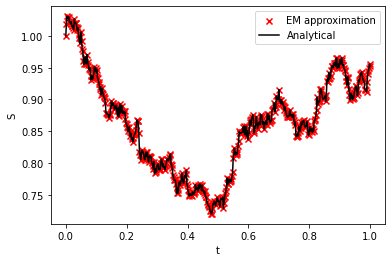
\includegraphics[width=0.48\textwidth]{graphics/em_simulation.png}
  \end{center}
  \caption{Realization of a EM approximated solution (eq. \ref{eq:EM}) compared to the analytical solution for the system in equation \ref{eq:system}.}
    \label{fig:em_vs_analytical}
\end{wrapfigure}

Let's consider the underlying Stochastic Differential Equation describing the time evolution of the \textit{option pricing}:

\begin{equation}\label{eq:system}
\begin{cases}
    dS(t) = rS(t)dt + \sigma S(t)dW_t &  t \in [0, T]\\
    S(0) = 1 &
\end{cases}
\end{equation}.

Here $dW_t$ refers to the differential of a standard \textit{Wiener process} $W_t$. We further define

\begin{equation}\label{eq:payoff}
    \mu := \E[Y] := \E[f(S)]
\end{equation}

for some given real functional $f$ applying to a stochastic process.
In our case of examination, $\mu$ will be the expected payoff at the final time $T = 1$, which will be the computational goal of this homework. 

In order to simplify the experiment, we will fix the values:

\begin{itemize}
\setlength\itemsep{0.05em}
\item The drift $r = 0.05$
\item The volatility $\sigma = 0.2$
\end{itemize}

%- \begin{math}Y = f(S(T))\end{math} is payoff at the final time.
%\\ -
%\begin{math}
%    T = 1
%\end{math} is the final time.
%\begin{math}
%     r = 0.05 
%\end{math} is the drift.
%\\ - 
%\begin{math}
%    \sigma = 0.2
%\end{math} is the volatility.
%\begin{math}W_t\end{math} a Standard Brownian Motion.
%\\ - \begin{math}\mu = \mathbb{E}(Y)\end{math} is the expected payoff.
%\\ - $K$ is the strike price.
%\\ - \begin{math}\epsilon\end{math} is the noise
%\\ - \begin{math}h\end{math} is the discretization parameter of the stochastic model

This system admits also an analytical solution as a log-normal stochastic process, which makes it easier to verify any other numerical solutions,

\begin{equation}\label{eq:system_analytical}
S(t) = \exp \left( (r - \frac{\sigma^2}{2})t + \sigma W_t \right)
\end{equation}.

\subsection{Time finite difference discretization}

The stochastic differential equation defined in eq. \ref{eq:system} can be discretized into a uniform grid $t_m = m h$ with $m = 1,\dots,M \in \N$, $T = Mh$, $h > 0$.
The first order approximation of the time derivative gives rise to the \textit{Euler-Maruyama} time discretization,

\begin{equation}\label{eq:EM}
\begin{cases}
    S_{m+1} = (1 + r h + \sigma \Delta W_m) \cdot S_m  & m = 1,\dots,M\\
    S_0 = 1
\end{cases}
\end{equation}

where $\Delta W_m \sim \mathcal{N}(0,h)$ is a $h$ increment of the Wiener process $W_t$.
The rate of convergence for this approximation is well known to be $\abs{\E[S_m] - \E[S(mh)]} = \mathcal{O}(t_m h)$ for the weak error and $\E[\abs{S_m - S(mh)}^p]^{\frac{1}{p}} = \mathcal{O}(t_m h^{\frac{1}{2}})$ for the strong error \cite{em}.

\subsection{Multi-level Monte Carlo Algorithm}

Now we want to build a Monte Carlo estimator of the expected payoff defined in equation \ref{eq:payoff} which efficiently computes the best approximation for any given function $f$. The special case we will consider in the next sections are going to be the \textit{Asian} option (eq. \ref{eq:asian}) and the \textit{Barrier call} option (eq. \ref{eq:barrier_call}).    
%In order to do so efficiently, \cite{} proposed a method that simulates $Y$ at different levels of discretization.
Let $\ell = 1,\dots,L \in \mathbb{N}$ denote the levels of simulation and $Y_\ell$, then the expectation can be decomposed in telescopic sum over different levels,

\begin{equation}\label{eq:expectation}
\mu = \mathbb{E}[Y_L] = \mathbb{E}[Y_0] + \sum_{\ell=1}^L \mathbb{E}[Y_\ell - Y_{\ell-1}] = \sum_{\ell=0}^L \mathbb{E}[Y_\ell - Y_{\ell-1}] 
\end{equation}

with $Y_{-1} = 0$ by convention.
Now approximate each expectation by a Monte Carlo estimator using $N_\ell$ samples for each independent level. This is called the multi-level Monte Carlo estimator and expresses as,

\begin{equation}\label{eq:MLMC}
\hat{\mu}_{MLMC} := \sum_{\ell = 0}^L \hat{\mu}_\ell = \sum_{\ell = 0}^L \frac{1}{N_\ell}\sum_{n=0}^{N_\ell} (Y_\ell^{(n,\ell)} - Y_{\ell - 1}^{(n,\ell)})
\end{equation}

with $\hat{\mu}_\ell$ is independent from $\hat{\mu}_k$ for $k \neq \ell$.
Furthermore, in order to minimize the variance of each level, $Y_\ell^{(n,\ell)}$ and $Y_{\ell - 1}^{(n,\ell)}$ must be simulated within the same underlying noise.
To do so, we will assume a discretization setup which decays exponentially as the level increases, i.e. fixing the first level discretization to $h_0$, the others will be $h_\ell = h_0 \cdot 2^{-\gamma\ell}$. For the sake of simplicity we will take $\gamma = 1$.

\paragraph{Joint Wiener process generation} \label{par:generation}
With this assumption, we can generate the same discretization grid which fits both for a level $\ell$ and its ancestor $\ell-1$. In particular, the generated noise is first sampled from a Wiener in the fine grained grid and then time differences $\Delta W_{\ell,m}^{(n,\ell)}$ are taken, with $m$ the time discretization index of the fine level.  
As those time differences are zero-mean normal distributed with variance $h$, then the coarser level's differences $\Delta W_{\ell-1,k}^{(n,\ell)}$, indexed by $k$, have variance $2h$. Assuming further both share the same points, i.e. $\Delta W_{\ell-1,k}^{(n,\ell)} = \Delta W_{\ell,m}^{(n,\ell)}$ for all $k = 2m$, then one finds an expression for the coarser level conditioned on the differences of the finer.

\begin{equation}\label{eq:browian_levels}
\Delta W_{\ell-1,k}^{(n,\ell)} = \Delta W_{\ell,m}^{(n,\ell)} + \Delta W_{\ell,m+1}^{(n,\ell)}, \quad \forall \; m = 2k
\end{equation}

\paragraph{MLMC Algorithm}
Finally, the algorithm for the Multi-level Monte Carlo is shown below:
\\
\\
\textbf{Inputs}: time steps $\{h_\ell\}_{\ell=0}^L$ and samples per level $\{N_\ell\}_{\ell=0}^L$
\begin{itemize}
    \item For \begin{math}\ell = 0 , ... , L\end{math}:
    \begin{itemize}

        \item For $n = 1, \dots , N_\ell$:

        \begin{itemize}
        
        \item Generate independent samples $\Delta W_{\ell,m}^{(n,\ell)} \sim \Normal(0, h_\ell)$ for $m = 0,\dots,(M_\ell -1)$
        \item Generate $\Delta W_{\ell-1,k}^{(n,\ell)}$ for $k = 0,\dots,(M_{\ell-1}-1)$ as shown in equation \ref{eq:browian_levels}.
        
        \item Simulate \begin{math}S_{\ell}^{(n,\,\ell)}\end{math} using EM with \begin{math}
            h = h_{\ell} ,\, \Delta \{W_{\ell,m}^{(n,\,\ell)}\}_{m=0}^{M_\ell-1}\end{math} as noise.
        \item Compute \begin{math}
                Y_{\ell}^{(n,\,\ell)} = f(S_{\ell}^{(n,\,\ell)})
            \end{math}


        \item If \begin{math}
            \ell > 0 
        \end{math}:

        \begin{itemize}
            \item Simulate \begin{math}S_{\ell-1}^{(n,\,\ell)}\end{math} using EM with \begin{math}
            h = h_{\ell-1} ,\, \{ \Delta W_{\ell-1,k}^{(n,\,\ell)} \}_{k=0}^{M_{\ell-1}-1} \end{math} as noise.
            \item Compute \begin{math}
                    Y_{\ell-1}^{(n,\,\ell)} = f(S_{\ell-1}^{(n,\,\ell)})
                \end{math}
            
        \end{itemize}

        \item Else, \begin{math}
            Y_{-1}^{(n ,\, \ell)} = 0
        \end{math}

        \end{itemize}
        
        \item Compute \begin{math}
            \hat{\mu}_{\ell} = \frac{1}{N_{\ell}} \sum\limits_{n = 1}^{N_{\ell}} ( Y_{\ell}^{(n,\,\ell)} - Y_{\ell-1}^{(n,\,\ell)} )
        \end{math}
    \end{itemize}
    \item Return \begin{math}\hat{\mu}_{L}^{MLMC} = \sum\limits_{\ell = 0}^{L} \hat{\mu}_{\ell} \end{math}
\end{itemize}

\subsection{Optimal sampling per level analysis (a)}

Let's denote $C_{MLMC}$ the overall cost of a run and $V_{MLMC}$ the variance achieved of the estimator $\hat{\mu}_{MLMC}$.
Furthermore, let's denote and $N_\ell$ the necessary number of samples which estimates $\mathbb{E}[Y_\ell - Y_{\ell-1}$, $C_\ell]$ the cost of the estimation procedure and $V_\ell$ the variance of the estimator. Considering that for each level $\ell$, $\hat{\mu}_\ell$ was previously defined as a Monte Carlo estimator using $N_\ell$ samples (eq. \ref{eq:MLMC}), the overall cost and variance express as,

\begin{align}\label{eq:mlmc_overall}
&C_{MLMC} = \sum_{\ell=0}^L N_\ell C_\ell &
&V_{MLMC} = \sum_{\ell=0}^L \frac{V_\ell}{N_\ell}
\end{align}

Our aim is to find the optimal number of samples per level $N_\ell$ such that the overall cost is fixed and the variance is minimized at the same time. Hence, in the \textit{Lagrange multipliers} formalism this reduces to find a constant $\lambda \in \mathbb{R}$ such that the following \textit{Lagrangian} expression is minimized,

\begin{equation}\label{eq:mlmc_lagrangian}
\mathcal{L}(N_1, \dots, N_L) = \sum_{\ell=0}^L \frac{V_\ell}{N_\ell} + \lambda \left( \sum_{\ell=0}^L N_\ell C_\ell  - C_{\varepsilon} \right)
\end{equation}

where $C_{\varepsilon}$ is the fixed cost.
By setting the gradient of the \textit{Lagrangian} to zero to find the minimum, one finds that the optimal number of samples per level is related to $\lambda$ by,

\begin{equation}\label{eq:mlmc_lambda}
N_\ell^* = \frac{1}{\sqrt{\lambda}}\sqrt{\frac{V_\ell}{C_\ell}}, \quad \text{for} \; \ell = 0,\dots,L 
\end{equation}.

Injecting this result into the overall variance expression one finds the optimal one at fixed cost, which can be bounded by a positive factor $\varepsilon^2$ representing an aimed fixed precision for all levels.

\begin{equation}\label{eq:mlmc_opt_variance}
\forall \; l=1,\dots,L \; : \;V_{MLMC}^* = \frac{1}{N_\ell^*}\sqrt{\frac{V_\ell}{C_\ell}} \left(\sum_{\ell=0}^L \sqrt{V_\ell C_\ell} \right) = \varepsilon^2
\end{equation}.

Hence, by taking $N_\ell^*$ as natural number, one finds its optimum,

\begin{equation}\label{eq:mlmc_opt_number}
N_\ell^* = \left\lceil \varepsilon^{-2} \sqrt{\frac{V_\ell}{C_\ell}} \left(\sum_{\ell=0}^L \sqrt{V_\ell C_\ell} \right) \right\rceil
\end{equation}.

